\documentclass{beamer}
\usepackage[utf8]{inputenc}

\usetheme{Madrid}
\usecolortheme{default}
\usepackage{amsmath,amssymb,amsfonts,amsthm}
\usepackage{txfonts}
\usepackage{tkz-euclide}
\usepackage{listings}
\usepackage{adjustbox}
\usepackage{array}
\usepackage{tabularx}
\usepackage{gvv}
\usepackage{lmodern}
\usepackage{circuitikz}
\usepackage{tikz}
\usepackage{graphicx}
\usepackage{multicol}
\setbeamertemplate{page number in head/foot}[totalframenumber]

\usepackage{tcolorbox}
\tcbuselibrary{minted,breakable,xparse,skins}



\definecolor{bg}{gray}{0.95}
\DeclareTCBListing{mintedbox}{O{}m!O{}}{%
  breakable=true,
  listing engine=minted,
  listing only,
  minted language=#2,
  minted style=default,
  minted options={%
    linenos,
    gobble=0,
    breaklines=true,
    breakafter=,,
    fontsize=\small,
    numbersep=8pt,
    #1},
  boxsep=0pt,
  left skip=0pt,
  right skip=0pt,
  left=25pt,
  right=0pt,
  top=3pt,
  bottom=3pt,
  arc=5pt,
  leftrule=0pt,
  rightrule=0pt,
  bottomrule=2pt,

  colback=bg,
  colframe=orange!70,
  enhanced,
  overlay={%
    \begin{tcbclipinterior}
    \fill[orange!20!white] (frame.south west) rectangle ([xshift=20pt]frame.north west);
    \end{tcbclipinterior}},
  #3,
}
\lstset{
    language=C,
    basicstyle=\ttfamily\small,
    keywordstyle=\color{blue},
    stringstyle=\color{orange},
    commentstyle=\color{green!60!black},
    numbers=left,
    numberstyle=\tiny\color{gray},
    breaklines=true,
    showstringspaces=false,
}
%------------------------------------------------------------
%This block of code defines the information to appear in the
%Title page
\title %optional
{10.3.11}
\date{October  2025}
%\subtitle{A short story}

\author % (optional)
{BEERAM MADHURI - EE25BTECH11012}



\begin{document}


\frame{\titlepage}
\begin{frame}{Question}
Find the normal at the point $(1,1)$ on the curve
\begin{align}
2y + x^2 = 3
\end{align}
\end{frame}

\begin{frame}{solution}
    \frametitle{finding the Normal:}
\begin{align}
    2y + x^2 = 3\\
    2y + x^2 -3 = 0
\end{align}
Which can be expressed as the conic:
\begin{align}
\vec{x^\top V x} + 2\vec{u^\top x} + f = 0\\
\vec{V} = \begin{pmatrix}1 & 0 \\0 & 0\end{pmatrix}, \vec{u} = \begin{pmatrix}0 \\1\end{pmatrix}, f = -3
\end{align}
\end{frame}
\begin{frame}
let 
\begin{align}
\vec{p} \begin{pmatrix} 1 \\ 1 \end{pmatrix} , \vec{m} \text{ is normal vector }\\
\vec{m}^\top \vec{(Vp + u)} = 0
\end{align}
substitung the value :
\begin{align}
\vec{m}=\begin{pmatrix} m_1 \\ m_2 \end{pmatrix} \\
\vec{Vp}=\begin{pmatrix}1 & 0 \\0 & 0\end{pmatrix}\begin{pmatrix}
    1\\1 \end{pmatrix}\\
    =\begin{pmatrix} 1\\0 \end{pmatrix}\\
\begin{pmatrix} m_1 \\ m_2 \end{pmatrix} \begin{pmatrix} 1+0\\0+1 \end{pmatrix}=0
\end{align}
\end{frame}
\begin{frame}
\begin{align}
m_1=-m_2\\
\therefore \vec{m}=\begin{pmatrix} -m \\ m \end{pmatrix}
\end{align}
equation of normal is
\begin{align}
    \vec{m}^\top(\vec{x-p})=0\\
    \begin{pmatrix} -1&1\end{pmatrix}\begin{pmatrix}x-1\\y-1   \end{pmatrix}=0\\
        y=x
\end{align}
Hence equation of normal to $2y + x^2 - 3 = 0$ at $(1,1)$ is $y = x$.
\end{frame}


\begin{frame}[fragile]
\frametitle{Python Code}
\begin{lstlisting}
import numpy as np
import matplotlib.pyplot as plt

# Create the figure and axis
fig, ax2 = plt.subplots()
fig.suptitle('Graphs of Normal to the Curve', fontsize=16)
# Curve: 2y + x^2 = 3  =>  y = (3 - x^2)/2
# Point: (1, 1)
# Normal Line: y = x
# Tangent Line at (1,1): y = -x + 2
\end{lstlisting}
\end{frame}

\begin{frame}[fragile]
\frametitle{Python Code}
\begin{lstlisting}
# Generate x-values for the curve
x_curve2 = np.linspace(-3, 4, 400)
y_curve2 = (3 - x_curve2**2) / 2

# Generate x-values for the lines
x_line2 = np.linspace(-2, 4, 100)
y_normal = x_line2
y_tangent2 = -x_line2 + 2
\end{lstlisting}
\end{frame}

\begin{frame}[fragile]
\frametitle{Python Code}
\begin{lstlisting}
# Plot the curve, normal, tangent, and the point
ax2.plot(x_curve2, y_curve2, label='Curve: $2y+x^2=3$', color='blue')
ax2.plot(x_line2, y_normal, label='Normal: $y=x$', color='green')
ax2.plot(x_line2, y_tangent2, label='Tangent: $y=-x+2$', color='red', linestyle='--')
ax2.scatter([1], [1], color='purple', s=100, zorder=5, label='Point (1, 1)')
\end{lstlisting}
\end{frame}

\begin{frame}[fragile]
\frametitle{Python Code}
\begin{lstlisting}
# Formatting for the plot
ax2.set_title('10.3.11: Normal to $2y+x^2=3$', fontsize=12)
ax2.set_xlabel('$x$')
ax2.set_ylabel('$y$')
ax2.axhline(0, color='black', linewidth=0.5)
ax2.axvline(0, color='black', linewidth=0.5)
ax2.grid(True, linestyle='--', alpha=0.7)
ax2.legend()
ax2.set_aspect('equal', adjustable='box')
ax2.set_xlim([-2, 4])
ax2.set_ylim([-2, 4])
\end{lstlisting}
\end{frame}

\begin{frame}[fragile]
\frametitle{Python Code}
\begin{lstlisting}
# Display the figure
plt.tight_layout(rect=[0, 0.03, 1, 0.95])
plt.show()
\end{lstlisting}
\end{frame}

\begin{frame}[fragile]
\frametitle{C Code}
\begin{lstlisting}
#include <stdio.h>

int main() {
    // --- Given Problem Data ---
    // The point (x1, y1) on the curve 2y + x^2 = 3.
    double x1 = 1.0;
    double y1 = 1.0;
    // --- Calculations ---
    // 1. Find the slope of the tangent from the derivative dy/dx = -x.
    double m_tangent = -x1;
\end{lstlisting}
\end{frame}

\begin{frame}[fragile]
\frametitle{C Code}
\begin{lstlisting}
    // A horizontal tangent (slope=0) means the normal is a vertical line.
    if (m_tangent == 0) {
        printf("The equation of the normal line is: x = %.2f\n", x1);
    } else {
        // 2. The slope of the normal is the negative reciprocal.
        double m_normal = -1.0 / m_tangent;
\end{lstlisting}
\end{frame}

\begin{frame}[fragile]
\frametitle{C Code}
\begin{lstlisting}
        // 3. The y-intercept 'c' is calculated from y = mx + c.
        double c = y1 - m_normal * x1;

        // --- Print the Final Answer ---
        // This logic helps format the equation cleanly (e.g., printing "y = x"
        // instead of "y = 1.00x + 0.00").
        printf("The equation of the normal line is: ");
\end{lstlisting}
\end{frame}

\begin{frame}[fragile]
\frametitle{C Code}
\begin{lstlisting}
        if (m_normal == 1 && c == 0) {
            printf("y = x\n");
        } else if (m_normal == -1 && c == 0) {
            printf("y = -x\n");
        } else {
            printf("y = %.2fx", m_normal);
            if (c > 0) {printf(" + %.2f\n", c);
            } else if (c < 0) {printf(" - %.2f\n", -c);
            } else {printf("\n");
            }}}
    return 0;}
\end{lstlisting}
\end{frame}

\begin{frame}[fragile]
\frametitle{Python and C Code}
\begin{lstlisting}
from ctypes import c_double

def main():
    # --- Given Problem Data ---
    x1 = c_double(1.0)
    y1 = c_double(1.0)

    # --- Calculations ---
    m_tangent = c_double(-x1.value)  # dy/dx = -x
\end{lstlisting}
\end{frame}

\begin{frame}[fragile]
\frametitle{Python and C Code}
\begin{lstlisting}
    if m_tangent.value == 0:
        print(f"The equation of the normal line is: x = {x1.value:.2f}")
    else:
        m_normal = c_double(-1.0 / m_tangent.value)
        c_intercept = c_double(y1.value - m_normal.value * x1.value)

        # --- Print the Final Answer ---
        print("The equation of the normal line is: ", end="")
\end{lstlisting}
\end{frame}

\begin{frame}[fragile]
\frametitle{Python and C Code}
\begin{lstlisting}
        if m_normal.value == 1 and c_intercept.value == 0:
            print("y = x")
        elif m_normal.value == -1 and c_intercept.value == 0:
            print("y = -x")
        else:
            print(f"y = {m_normal.value:.2f}x", end="")
            if c_intercept.value > 0:
                print(f" + {c_intercept.value:.2f}")
\end{lstlisting}
\end{frame}

\begin{frame}[fragile]
\frametitle{Python and C Code}
\begin{lstlisting}
            elif c_intercept.value < 0:
                print(f" - {abs(c_intercept.value):.2f}")
            else:
                print()

if __name__ == "__main__":
    main()

\end{lstlisting}
\end{frame}
\begin{frame}
\begin{figure}[H]
    \centering
    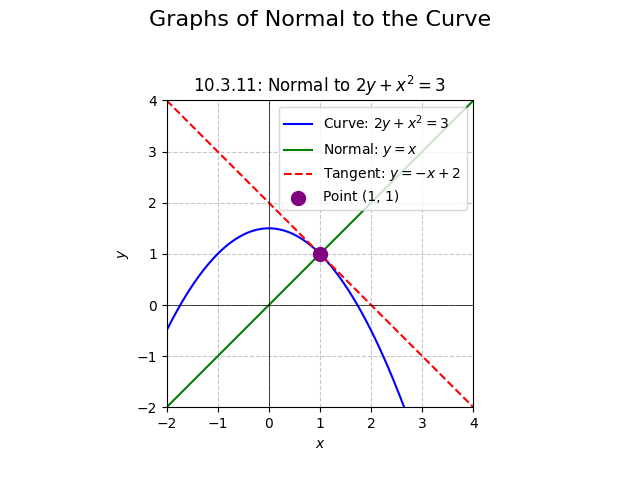
\includegraphics[width=0.75\columnwidth]{graph-17.png}
    \caption{Plot}
    \label{fig:placeholder}
\end{figure}
\end{frame}

\end{document}